Um die Frage zu beantworten wie man zwei SQL Anfragen miteinander vergleichen kann, muss man sich zunächst die Struktur einer solchen Anfrage betrachten. Exemplarisch betrachten wir im folgenden \verb|SELECT| Anfragen. Es werden mehrere Ansätze in diesem Teil der Arbeit verfolgt, wie man die Gleichheit von zwei Anfragen zeigen kann. Offensichtlich sind zwei SQL-Anfragen semantisch äquivalent, wenn sie ebenfalls syntaktisch korrekt sind. Interessanter sind daher Anfragen, die zunächst nicht syntaktisch dekungsgleich sind. 

Ein Ansatz besteht darin beide SQL-Anfragen einer Standardisierung zu unterziehen. Wie genau so etwas durchgeführt werden kann, wird im Folgenden noch erläutert. Wir würden dann zwei standardisierte SQL-Anfragen erhalten. Sind diese syntaktisch äquivalent, so handelt es sich um identische Anfragen. Dieser Ansatz wird uns mit einigen Problemen konfrontieren und daraus entwickeln wir einen zweiten Ansatz. 

Dieser versucht durch gleichartige Umformungen, die zwei Anfragen zu unifizieren (gleich zu machen). Bei diesem Ansatz würden wir also versuchen die geparsten Operatorbäume miteinander zu vergleichen. Auch diese Lösung birgt Vorteile aber auch Probleme mit sich, die im Folgenden besprochen werden.

\section{Hintergrund}

Es gibt syntaktisch unterschiedliche Anfragen, die jedoch semantisch äquivalent sind. So liefern die folgenden Anfragen die gleichen Ergebnisse, sind aber nicht syntaktisch äquivalent.

\begin{verbatim}
SELECT * FROM emp e WHERE e.enr > 5
\end{verbatim}

\begin{verbatim}
SELECT * FROM emp e WHERE 5 < e.enr
\end{verbatim}

\begin{verbatim}
SELECT * FROM emp e WHERE e.enr >= 6
\end{verbatim}

Wie man leicht sieht, sind die Anfragen ähnlich. Im folgenden werden zwei Strategien besprochen, welche beide zum Ziel haben, zwei SQL-Anfragen miteinander zu vergleichen.

\section{Workflow}

\begin{verbatim}
INPUT: QUERY Q1,Q2;
P1 = preprocessing(Q1);
P2 = preprocessing(Q2);
compare(P1,P2); // possible warnings can be displayed now
ANSWER = match(Q1,Q2);
if ANSWER yes then
    /* If that worked, we know both solutions are the same */
    display success
else 
    if do_real_db_compare(Q1,Q2) then
        /* now we don't know if they are the same because
         * they couldn't be matched but test on real data 
         * showed the correct results 
         display may be correct
    else 
        /* if the real data test failed we have a proof 
         * in form of a data set, that both querys can't be the same */
         display fail
    endif
endif
output result of compare(P1,P2)
/* The result may show the cause of a fail or a ``may be'' solution. 
 * It can provide hints so that the student can improve.
 * Even if the solution was correct i.e. it was matched with the sample solution, 
 * it may be that the students soltion contained unnecassary joins, or formulas. */
\end{verbatim}

\section{Preprocessing}

Im Abschitt >>Forschungsstand<< haben wir bereits einige Lernplattformen/projekte zum Thema SQL kennen gelernt. Viele dieser Plattformen möchten dem Lernenden genügend Feedback beim Lernprozess geben. Dies ist nicht nur sinnvoll, damit der Student schneller auf korrekte Lösungen stößt, sonder auch, weil die Standardhinweise eines SQL Systems meist nur auf syntaktische Fehler hinweisen. Einen großen Beitrag zur Verbesserung von Fehlermeldungen hat das Projekt SQLLint vorzuweisen, da es Fehlermeldungen und Hinweise konkreterer Natur ausgibt. Hervorzuheben ist, noch einmal, dass es sich hierbei um semantische Fehlermeldungen handelt. Schon nach kurzer Einlernzeit sinken die Anzahl an syntaktischen Fehlern bei Lernenden. Dafür machen diese mehr semantische Fehler, was um so schlimmer ist, da bisher kaum oder keine Warnhinweise für solche Fehler existierten. 

Dennoch sollen in dieser Arbeit zwei SQL-Anfragen verglichen werden. Wir können hier also nicht alle Ideen des SQLLint übernehmen. Egal ob das Matchen der Musterlösung und der Lösung des Lernenden gelingt oder nicht, wir möchten dem Lernenden Feedback geben, an dem er möglicherweise sehen kann, warum das Matching nicht gelungen ist. Wir können dabei, wie bereits erwähnt, nicht an die Komplexität des SQLLint anknüpfen. Stattdessen werden wir uns eines einfachen Sammelns von Metainformationen der SQL-Anfrage bedienen. Diese sammeln wir bevor die zwei Anfragen durch Folgeschritte angepasst oder verändert werden. Am Ende des Matchingsversuchs sollen Metainformationen der zwei Anfragen verglichen werden und dem Lernenden soll Feedback gegeben werden. Konnte keine Übereinstimmung der zwei Anfragen erreicht werden, so können die Metainformationen dem Lernenden Anhaltspunkte für eine richtige Lösung geben. Konnten die Anfragen unifiziert werden, so sind die Metainformationen dennoch von Interesse. Es könnte sein, dass der Lernende eine unnötig komplexe Lösung eingesandt hat, die sich durch Anpassungen vereinfachen ließe. So kann der Lernende potentiell auch aus einer korrekten Lösung noch etwas lernen.

Wir möchten für jede SQL-Anfrage ein Preprocessing vor der eigentlichen Bearbeitung vorschalten, was im wesentlichen folgende Punkte beinhalten soll.

\begin{itemize}
\item Anzahl der JOIN Bedingungen
	\begin{itemize}
	\item Anzahl von OUTER/INNER Joins
	\end{itemize}
\item Anzahl atomarer Formeln in \verb|WHERE|-Teil
\item Anzahl atomarer Formeln in \verb|HAVING|-Teil
\item Anzahl Tabellen in \verb|FROM|-Teil
\item Anzahl Attribute im \verb|SELECT|-Teil *
\item existiert ein \verb|DISTINCT|
\item existiert ein \verb|GROUP BY| *
	\begin{itemize}
	\item wenn ja, stimmen die Attribute überein?
	\end{itemize}	 
\item existiert ein \verb|HAVING BY|
\item existiert ein \verb|ORDER BY| und ist es notwendig? (\verb|ORDER BY ... ASC|) *
\item Tiefe des Parserbaums, kann Aufschluss über unnötige Klammerung geben. Siehe dazu Abschnitt >>Wie funktioniert der Parser<<
\end{itemize}

Unterscheiden sich Musterlösung und Lösung des Studenten in den mit * markierten Punkten ist es extrem unwahrscheinlich, dass beide Lösungen die gleichen Tupel zurückliefern würden. Hier möchten wir im Vorfeld dem Lerneden eine Warnung anzeigen, dass er höchstwahrscheinlich etwas vergessen hat. Alle anderen Punkte werden im Anschluss an die eigentliche Analyse der Anfragen abgeglichen. So sind etwa folgende Meldungen denkbar:

\begin{itemize}
\item ``the sample solution contains two joins but your solution does not contain any join.''
\item ``Your solution is correct but the sample solution contains two less atomar formulas (formula1, formula2).''
\item ``Your solution is correct but the sample solution does not contain DISTINCT. Reconsidder if it is really necessary.''
\end{itemize}

\section{Standardisierung von SQL-Anfragen}

Zunächst verfolgen wir den Ansatz zwei SQL-Anfragen zu vergleichen, indem wir sie standardisieren. Die Kriterien der Standardisierung werden im Detail behandelt. Standardisiert man die Musterlösung, als auch die Lösung des Lernenden nach den gleichen Kriterien, so kann man danach durch einen einfachen Stringvergleich auf die Äquivalenz schließen. 

\subsection{Entfernen von syntaktischen Details}

Das Entfernen von syntaktischen Details übernimmt zum großen Teil bereits der Parser. Er entfernt unnötige Leerzeichen, Kommentare sowie unnötige Klammern. Aufgrund der Arbeitsweise des Parsers gibt es allerdings Situationen, in dem der Parser scheinbar nicht alle unnötigen Klammern entfernt. Wie im Abschnitt >>Verwendeter Parser<< erläutert wird, sind die geparsten Bäume nicht binär. Ein Baum wie in Abbildung \ref{baum1} zu sehen, ist daher zu vermeiden. 

Der Parser hilft allerdings dabei die SQL-Anfrage in einer Datenstruktur zu überführen, die frei von allen syntaktischen Details ist. Dazu gehören Leerzeichen, Tabs, Zeilenumbrüche und Groß/Kleinschreibung von Schlüsselwörtern.

\subsection{Vereinheitlichen der FROM Klausel}

Wir beginnen mit der Betrachtung der \verb|FROM| Klausel. Da die Reihenfolge der Spaltennamen im \verb|SELECT| Teil oft von der Aufgabenstellung vorgeschrieben ist, wird diese auch nicht verändert.

Im \verb|FROM| Teil werden zunächst alle auftretenden Tabellennamen lexikographisch sortiert. Danach werden automatische Aliase erzeugt. Sind bereits Aliase vergeben wurden, so werden diese ebenfalls durch die automatischen Aliase ersetzt. Eine Hashtabelle speichert frühere Zuweisungen, damit im \verb|SELECT| und \verb|WHERE| die Aliase ebenfalls korrekt ersetzt werden.

Hatten die vorkommenden Tabellen im \verb|FROM| Teil keinen Alias wird nur der küsntliche Alias eingeführt.

\begin{figure}
Eingabe: \\\verb|SELECT e.id, e.name, d.region FROM emp e, dep d WHERE e.depid = d.id|\\

Anpassung: \\\verb|SELECT a2.id, a2.name, a1.region FROM dep a1, emp a2 WHERE a2.depid = a1.id|\\
\caption{Beispiel: Umwandlung des FROM Teils einer SQL-Anfrage}
\end{figure}

\subsection{Umwandlung der WHERE Bedingung in KNF}

Aufgrund der Eigenheiten des ZQL-Parsers ist es möglich, dass eine unnötige Klammerung nicht entfernt wird. Beispiele dafür sind im Abschnitt >>ZQL-Parser<< zu finden. Es ist daher wünschenswert eine Normalform des \verb|WHERE| Teils zu erreichen. In diesem Fall wurde die konjunktive Normalform (KNF) gewählt.


\subsubsection{Entfernung unnötiger Klammerungen}

Ein Ausdruck \verb|((a > 5)  and ((b > 5) and (c > 5)))| enthält unnötige Klammern, da der Operator \verb|and| als Operand von einem weiteren \verb|and| vorkommt. Folgender Ausdruck ist äquivalent: \verb|((a > 5)  and (b > 5) and (c > 5))|. Diese spezielle Form der Klammerung entsteht aus der Tatsache, dass der ZQL-Parserbaum nicht binär ist und beide,  eben genannten, Beispiele nicht den gleichen Baum beschreiben. Als ersten Schritt in Richtung KNF möchten wir solchen unnötigen Klammern entfernen. 

Es ist daher wünschenswert, wenn ein Operator X einen Ausdruck als Kindknoten besitzt, in dem X ebenfalls der Operator ist, den Operator X im Kindknoten zu eliminieren und alle Kinder vom eliminierten Kindknoten an den verbleibenden Operatorknoten X zu hängen. Damit hätte man den Ausdruck vereinfacht, da die assoziative Klammerung wegfällt. Wir nennen dieses Vorgehen im Folgenden Operatorkompression.

Gegeben sei der ZQL-Parsebaum $B=(V,E)$. Es sei $child(v) = \{ w : w\in V \wedge (v,w)\in E\}$, also die Menge aller Kindknoten von $v$. Gibt es einen Knoten $w\in child(v)$ mit $v=w$, so wird Knoten $w$ eliminiert und alle Kindknoten von $w$ werden zu Kindknoten von $v$, also $child(v) = child(v) \cup child(w)$. 
$E=E\backslash \{ (w,x) : x\in child(w)\} \cup \{(v,x) x\in child(w)\}$ und $V=V\backslash \{w\}$.

Im Sinne des Vergleiches der Komplexität der Musterlösung mit der Komplexität der Lösung des Lernenden ist es sinnvoll zu speichern, ob und wie oft eine solche Operatorkompression durchgeführt werden musste.

\subsubsection{NOT auflösen}

Im nächsten Schritt möchten wir auftretende \verb|NOT| Operatoren entfernen. Dies geschieht indem der Operator \verb|NOT| im Parserbaum nach unten geschoben wird. Dabei werden die \textit{DE MORGAN} Regeln angewendet. 

\begin{tabular}{ll}
Eingabe: & Umwandlung Teil 1:\\
\verb|not ((a > 5)  and ((b > 5) or (c > 5)))| & \verb|(not(a > 5) or not((b > 5) or (c > 5)))|\\
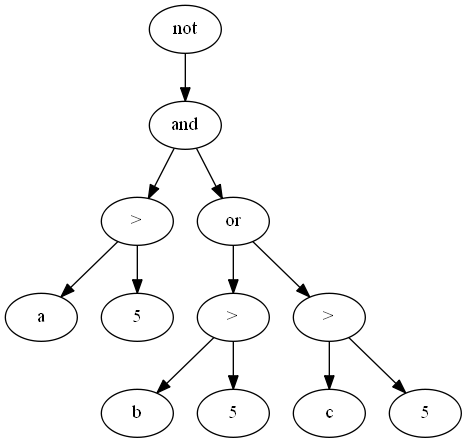
\includegraphics[scale=0.5]{Bilder/not_graph1.png} & 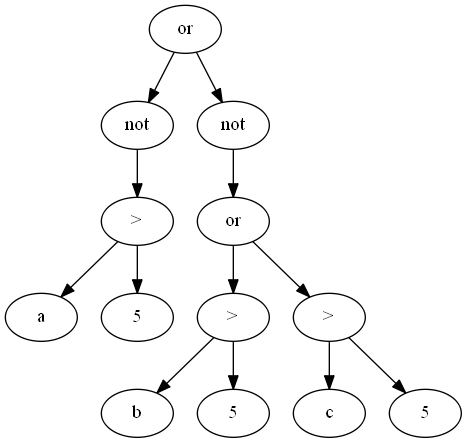
\includegraphics[scale=0.5]{Bilder/not_graph2.png}\\
\end{tabular}

\begin{tabular}{ll}
Umwandlung Teil 2: & Umwandlung Teil 3:\\
\verb|((a <= 5) or (not(b > 5) and not(c > 5)))| & \verb|((a <= 5) or ((b <= 5) and (c <= 5)))|\\
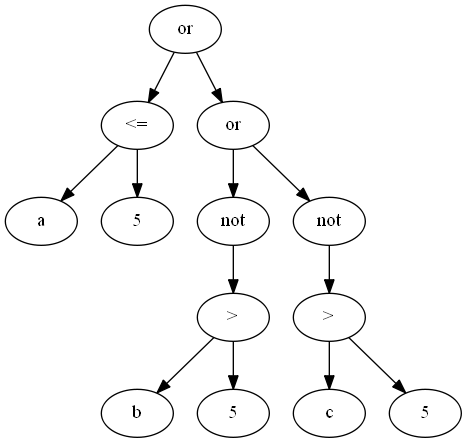
\includegraphics[scale=0.5]{Bilder/not_graph3.png} & 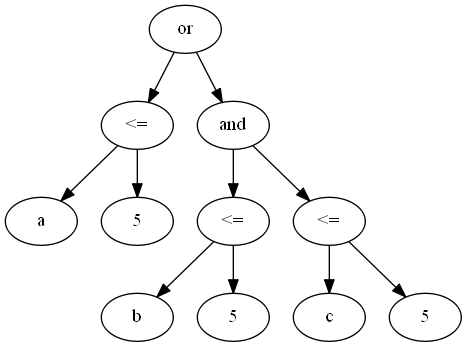
\includegraphics[scale=0.5]{Bilder/not_graph4.png}\\
\end{tabular}


\subsubsection{Anwenden des Distributivgesetzes}

Im letzten Schritt haben wir die Formel \verb|((a <= 5) or ((b <= 5) and (c <= 5)))| erhalten. Durch Anwenden des Distributivgesetzes können wir diese Formel im letzten Schritt umformen zu: \verb|((a <= 5) or (b <= 5)) and ((a <= 5) or (c <= 5))|

\subsection{Ersetzung von syntaktischen Varianten}

Um eine Anfrage zu standardisieren müssen wir den syntaktischen Zucker entfernen. Dies geschieht, in dem man nur eine syntaktische Schreibweise anerkennt und alle anderen Schreibweisen werden in die zulässige umgewandelt. Zu erwähnen sind folgende Ersetzungen, die durchgeführt werden sollen um syntaktisch vielfältige, aber semantisch äquivalente Ausdrücke zu minimieren.

\begin{figure}
\begin{tabular}{ccl}
\verb|A BETWEEN B AND C| & $\to$  & \verb|A >= B AND A <= C|\\
\verb|SELECT ALL| & $\to$ & \verb|SELECT|\\
\verb|ORDER BY VAR ASC| &  $\to$ & \verb|ORDER BY VAR|\\
\verb|EXISTS (SELECT A,B,C ...)| & $\to$ & \verb|EXISTS (SELECT 1 ...)|\\
\end{tabular}
\caption{Entfernen von syntaktischen Varianten}
\end{figure}

Ein \verb|INNER JOIN| kann sowohl im \verb|FROM|, als auch im \verb|WHERE| Teil einer SQL-Anfrage formuliert werden. Damit Untersuchungen einheitlich geschehen können, formulieren wir solche JOINs im \verb|WHERE| Teil der SQL-Anfrage.

\begin{figure}
Eingabe:\\
\verb|SELECT * FROM foo f INNER JOIN bar b ON f.id=b.id|\\

Umwandlung:\\
\verb|SELECT * FROM foo f, bar b WHERE f.id=b.id|\\
\caption{Umwandlung von INNER-JOIN}
\end{figure}

Bei Anwendung dieser Ersetzungsregeln, soll dem Lernenden ein klares Feedback gegeben werden. Es soll verdeutlicht werden, dass eine korrekte Anfrage dennoch Mängel aufweist, da unnötige Formulierungen benutzt wurden.

Eventuell ist es hier auch bereits möglich Terme, die nur aus numerischen Konstanten bestehen zu Ersetzen durch das jeweilige Ergebnisse. So könnten arithmetische Operationen bereits ausgeführt und Vergleiche, die nur aus numerischen Konstanten bestehen, durch entsprechende Wahrheitswerte ersetzt werden.

\subsection{Operatorenvielfalt}

Im folgenden Abschnitt soll geklärt werden wie mit verschiedenen Schreibweisen von ein und demselben Ausdruck umgegangen werden soll. Betrachtet man sich zum Beispiel: \verb|A > 5| ist dieser Ausdruck äquivalent mit \verb|5 < A|. Wenn wir wissen, dass \verb|A| ein ganzzahlige Variable ist, dann sind auch folgende Äquivalenzen wahr: \verb|A >= 6| so wie \verb|6 <= A|. Wir betrachten nun zwei verschiedene Ansätze um mit diesem Problem umzugehen. Ein Ansatz beschäftigt sich damit, alle implizierten Schreibweisen mit in die Formel aufzunehmen. Damit stellt man sicher, dass sich alle korrekten Schreibweisen einer Formel in der Anfrage befinden. Der zweite Ansatz beschäftigt sich damit, nur bestimmte Schreibweisen zuzulassen und alle anderen durch die zulässigen zu ersetzen.

Hinweis: Diesem Schritt geht eine Teilsortierung vor. Diese wird ebenfalls im Abschnitt >>Sortierung<< erwähnt. 

\subsubsection{Teilsortierung}

Wir betrachten Ausdrücke mit den Operatoren $\{>,<,\leq,\geq,=,+,\cdot\}$. Da es sich hier jeweils um binäre Operatoren handelt, sprechen wir -- im Sinne der Anordnung -- im Folgenden von einem linken und einem rechten Operanden. Ist einer der Operanden eine Variable, so wird diese links angeordnet. Sind beide Operanden Variablen, so werden sie lexikographisch-sortiert angeordnet. Operanden, die selbst wieder zusammengesetzte Ausdrücke sind, stehen rechts. Sind beide Operanden zusammengesetzte Ausdrücke, so steht der komplexere rechts und der weniger komplexe links. Ein Ausdruck $A$ ist komplexer als ein Ausdruck $B$, wenn der zugehörige Operatorbaum von $A$ tiefer ist als der Operatorbaum von $B$. Sind beide Ausdrücke gleich komplex, so wird die symmetrische Variante mit hinzugenommen. Wenn wir Operanden umsortieren bei denen der Operator $\in \{>,<,\leq,\geq\}$ ist, dann muss der jeweilige Operator auch umgedreht werden. Bei den restlichen Operatoren ist dies nicht der Fall, da diese symmetrisch sind.

\subsubsection{Hinzufügen implizierter Formeln}

Trifft man im Parserbaum auf eine Formel, zu der es mehrere äquivalente Formeln gibt, so ist ein Ansatz alle diese äquivalenten Formeln konjunktiv zu verknüpfen und mit in den Parserbaum aufzunehmen. Treffen wir also zum Beispiel auf folgenden Ausdruck \begin{verbatim}SELECT * FROM testtable WHERE A = B - C\end{verbatim}, so müssen wir auch alle äquivalenten Formeln mit aufnehmen. Daraus wird dann also der Ausdruck: \begin{verbatim}...WHERE A = B - C AND B = A + C AND C = B - A\end{verbatim}

Wie man bereits sieht, sind die hinzugefügten Formeln redundant und tragen nicht effizient zur Beschleunigung der Anfrage bei. Es soll hier lediglich sichergestellt werden, dass alle möglichen äquivalenten Formeln auftreten, da wir nicht wissen, was der Student für einen Repräsentanten der Formeln wählen wird. Weiterhin muss bemerkt werden, dass dadurch die gesamte SQL-Anfrage enorm aufgebläht wird. Es ist daher unbedingt wichtig, die Originalanfrage zu speichern. Weiterhin muss das Programm eine Verbindung zwischen den Formeln der Originalanfrage und den Formeln der veränderten, aufgeblähten Anfrage herstellen. Dem Lernenden soll in einem Feedback nur Fehler in der Originalanfrage aufgezeigt werden. Da intern aber mit der aufgeblähten Anfrage gearbeitet wird, muss beim Auftreten eines Fehlers oder Hinweises nachgeschlagen werden, von welchem Teil der Originalanfrage der Teil entstammt, der jetzt den Fehler auslöst.

Im Folgenden listen wir Mengen $M_i$ von Ausdrücken. Finden wir in der zu bearbeitenden SQL-Anfrage eine Formel $f$, die auf einen Ausdruck $a\in M_i$ passt, dann verknüpfen wir alle Ausdrücke $\{b : b\in M_i \wedge b \neq a\}$ konjunktiv mit $f$.

Im folgenden sind alle Variablennamen $A,B,C$ keine (komplexe) Ausrücke. Es handelt sich also jeweils um Blattknoten im Parserbaum. Ferner bezeichnen wir $X,Y$ als numerische Konstanten.\\

\begin{tabular}{ll}
$M_1$ & $\{\ A=B-C\ ,\ C=B-A\ ,\ B=A+C\ \}$\\
$M_2$ & $\{\ A=B\cdot C\ ,\ C=A / B\ ,\ B=A / C\ \}$\\
$M_3$ & $\{\ A>B-C\ ,\ C>B-A\ ,\ B<A+C\ \}$\\
$M_4$ & $\{\ A<B-C\ ,\ C<B-A\ ,\ B>A+C\ \}$\\
$M_5$ & $\{\ A>B, B<A \}$\\
$M_6$ & $\{\ A\geq B, B\leq A \}$\\
$M_7$ & $\{\ A>X, A\geq X+\mathit{adjust}(A) \}$\\
$M_8$ & $\{\ A<X, A\leq X-\mathit{adjust}(A) \}$\\

\end{tabular}

Beim Vergleich mit $>$ und $<$ ist es wichtig zu wissen, wie viel Nachkommastellen die numerischen Variablen $A$ und $B$ besitzen. Es sei $\mathit{places}(A)$ die Anzahl der Nachkommastellen der Zahl $A$. Dann bezeichnen wir mit $\mathit{adjust}(A) = 1 / (10^{\mathit{places}(A)})$, einen angepassten Wert, der sich nach der Stelligkeit der Variable A richtet.

Finden wir Ausdrücke mit $>,<,\leq,\geq$, welche als Argumente Variablen oder Konstanten haben, so unterscheiden wir grundsätzlich 3 Fälle.

Fall 1 $(M_5,M_6)$: Beide Operanden sind Variablen. In diesem Fall ergänzen wir nur den jeweils symetrischen Operator. Da beide Operanden Variablen sind, macht es keinen Sinn jeweils $\leq,\geq$ oder $<,>$ zu ersetzen.

Fall 2 $(M_7,M_8)$: Einer der beiden Operanden ist eine numerische Konstante. In diesem Fall fügen wir alle implizierten Gleichungen hinzu, also insbesondere die Operatoren $\leq,\geq,<,>$. Zu beachten ist hier, dass nicht nur Gleichungen der Form $A>X$ dazu führen, dass alle Ausdrücke von $M_7$ hinzugefügt werden. Auch wenn eine Gleichung der Form $Var1\geq 5.2$ auftaucht werden Ersetzungen durchgeführt. Diese Gleichung passt auf das Muster $A\geq X+\mathit{adjust}(A)$. Angenommen $Var1$ hat maximal eine Nachkommastelle, so würden dann folgende Gleichungen impliziert werden: $\{\ Var1>5.1\ ,\ 5.1<Var1\ ,\ 5.2 \leq Var1\ \}$.

Fall 3: Beide Operanden sind numerische Konstanten. In dem Fall wird die logische Aussage ausgewertet und durch ihren Wahrheitswert ersetzt [0,1].

Sind durch die hinzugefügten Terme nun arithmetische Ausdrücke entstanden, die nur noch numerische Konstanten enthalten, so werden diese Ausdrücke ausgewertet.

Dieser Teilschritt erfordert weiterhin eine Sortierung der einzelnen Terme.

\subsubsection{Beschränkung der Operatorenvielfalt}

Ein weiterer Ansatz das Problem der äquivalenten Formeln anzugehen ist es, bestimmte Operatoren zu >>verbieten<<. Das soll bedeuten, wir definieren verbotene Operatoren, welche am Ende der Umwandlungen nicht mehr in der SQL-Anfrage vorkommen dürfen. Dies wird erreicht, indem wir jeden verbotenen Operator umwandeln in einen nicht-verbotenen Operator. Das Prinzip ähnelt dem eben Vorgestelltem. Wir betrachten uns wieder die Mengen $M_i$. Des Weiteren hat jede Menge $M_i$ einen Repräsentanten $r(M_i)$. Finden wir nun in der zu bearbeitenden Anfrage eine Formel $f$, die auf eine der Ausdrücke $a\in M_i$ passt, so ersetzen wir $f$ mit $r(M_i)$. Folgende Tabelle soll die Mengen und deren Repräsentanten beschreiben:

\begin{tabular}{lll}
$i$ & $M_i$ & $r(M_i)$ \\
$1$ & $\{\ A=B-C\ ,\ C=B-A\ ,\ B=A+C\ \}$ & $B=A+C$\\
$2$ & $\{\ A=B\cdot C\ ,\ C=A / B\ ,\ B=A / C\ \}$ & $A=B\cdot C$\\
$3$ & $\{\ A>B\ ,\ B<A,A\geq B+\mathit{adjust}(B)\ ,\ B\leq A - \mathit{adjust}(A)\ \}$ & TODO\\
\end{tabular}

Im Folgenden soll ein Beispiel die Prozedur verdeutlichen.\\

Es sei unsere Ausgangsanfrage: \begin{verbatim}SELECT * FROM testtable WHERE X = 6 - Y\end{verbatim}

Die Formel $X=6-Y$ finden wir in $M_1$ in Form von $A=B-C$. Wir ersetzen nun also $X=6-Y$ mit dem Repräsentanten von $M_1$, und wir bekommen: \begin{verbatim}SELECT * FROM testtable WHERE 6 = X + Y\end{verbatim}

\subsubsection{Diskussion der beiden Ansätze}

Ein wesentlicher Punkt beim Vergleich beider Ansätze ist der Aufwand bzw. die Laufzeit beider Ansätze. 

Betrachten wir zunächst den Ansatz des Hinzufügens von implizierten Formeln. Wir müssen in einer Tiefensuche jede Formel betrachten und mit allen Mengen $M_i$ abarbeiten. Finden wir in einer Menge ein Muster wieder, so wird unsere Formel künstlich aufgebläht. Wir haben also für das Suchen eine maximale Laufzeit von $\mathcal{O}(\mathit{\vert Formeln\vert \cdot max\{i : M_i\}})$. Das Einfügen der Formeln geschieht in konstanter Zeit $\mathcal{O}(1)$, da wir ja immer eine konstante Anzahl an Formeln ergänzen.

Beim anderen Ansatz werden bestimmte Operatoren verboten. Wir realisieren dieses Verbot wieder über eine Suche. Es muss auch hier jede Formel auf ein Muster in $M_i$ untersucht werden. Wir benötigen für das Suchen in diesem Ansatz also genau so viel Zeit, wie im ersten Ansatz. Auch das Ersetzen der Formeln hat keine Zeitersparnis gegenüber einem Hinzufügen von weiteren Formeln. Es muss bemerkt werden, dass in diesem Fall die Originalformel nicht weiter aufgebläht wird.

Da sich die Laufzeiten der beiden Varianten nicht unterscheiden, müssen andere Kriterien zum Vergleich herangezogen werden. Wichtig für Software ist nicht ausschließlich die Laufzeit, sondern auch die Wartbarkeit. Besonders bei Projekten, die im Rahmen einer Masterarbeit entstehen, ist es wahrscheinlich, dass der Autor sich später nicht mehr um das Projekt kümmern kann. Daher sollte man sich bei den hier vorliegenden Ansätzen fragen, welcher leichter wartbar und erweiterbar ist.

Muss das Programm erweitert werden und wir möchten den Ansatz des Hinzufügen implizierter Gleichungen verwenden, so muss lediglich eine weitere Menge $M_k$ erstellt werden. Der Algorithmus sucht automatisch, dann auch in dieser neuen Menge nach Mustern und würde alle anderen Elemente dieser Menge konjunktiv-verknüpft zur Formel hinzufügen. 

Bei der Verwendung von eingeschränkten Operatoren gestaltet sich dieser Ansatz bereits als schwierig. Hier muss man nicht nur die neue Menge $M_k$ angeben, sondern sich auch Gedanken machen, was ein geeigneter Repräsentant dieser Menge ist. Unter Umständen kann das Auswählen eines ungünstigen Repräsentanten zu unerwarteten Problemen, wie dem Verkomplizieren der Anfrage, führen.

Es bietet sich aus diesen Umständen eher an, das Hinzufügen von implizierten Gleichungen zu verwenden.

\subsection{Sortierung}

Im aktuell betrachteten Ansatz möchten wir zwei Anfragen dadurch vergleichen, dass wir sowohl die Musterlösung, als auch die Studentenlösung einer Standardisierung unterziehen. Ein ganz wesentlicher Aspekt dabei ist, die Art der Sortierung. Sind die ZQL-Parserbäume isomorph zueinander, dann lässt sich das leicht zeigen, in dem man beide nach gleichartigen Kriterien sortiert und dann einen direkten Abgleich vornimmt.

Dabei unterscheiden wir zwei Arten von Sortierung. Hat ein Operator als Operanden nur Ausdrücke und keine Konstanten oder Variablen dann sortieren wir die Kindknoten, welche jeweils wieder eigene Terme bilden.

Hat ein Operator als Operand mindestens eine Konstante oder Variable, so Sortieren wir das innere dieses Terms.

\subsubsection{Sortierung im Inneren der Terme}

Hat ein Operator \textit{OP1} als Kindknoten mindestens ein Blatt, dann werden die Kindknoten so sortiert, dass zunächst die Blattknoten (lexikographisch) und erst dann die Teilbäume erscheinen. Möglich wird dies, weil die Tabellen-Aliase in einem vorherigen Schritt bereits automatisch sortiert und benannt wurden. Bei symmetrischen Operatoren wie $=,  \textit{AND}, \textit{OR}$ können die Kindknoten einfach umgehangen/umsortiert werden. Bei Operatoren wie $\le,\ge$ ist es notwendig den Operator \textit{OP1} umzudrehen. Weil aber die Sortierung außerhalb von Termen auf den Operatoren basiert, ist es notwendig, die Sortierung im Inneren der Terme zuerst durchzuführen.

Dieser Schritt wurde bereits als Vorbereitung der Schritte >>Hinzufügen von implizierten Formeln<< und >>Operatorbeschränkung<< durchgeführt. 

\subsubsection{Sortierung von Termen}

Hat ein Operator \textit{OP1} als Kindknoten nur weitere Operatoren \textit{OP2,OP3}, dann muss anhand dieser Operatoren die Reihenfolge im Baum festegelegt werden. Dies geschieht, in dem wir uns einfach eine Reihenfolge der Operatoren ausdenken. Wir überlegen uns folgende Ordnung $order:\textit{Relation}\to\mathbb{N}$, in der eine Relation $r$ vor einer Relation $s$ im standardisierten Parserbaum erscheint, wenn $order(r) < order(s)$.

$order:$\\

\begin{tabular}{|llllllll|}
\hline
$r\in \textit{Relation}$ & $\le$ & $\ge$ & $>$ & $<$ & $=$ & IS NULL & IS NOT NULL  \\
$\textit{order}(r)$ & 1 & 2 & 3 & 4 & 5 & 6 & 7\\ 
\hline
\end{tabular}\\

Es sei $\textit{RT}(\textit{OP})$ der Teilbaum des SQL-Ausdruckes mit der Wurzel \textit{OP}. Wir bezeichnen mit $\textit{depth}(\textit{RT}(\textit{OP}))$ die Tiefe des Baumes $\textit{RT}(\textit{OP})$. Es seien $\textit{child}(\textit{OP}) = \{v_1,v_2,...,v_i,...,v_n\}$ die Kindknoten von $\textit{OP}$. Die korrespondierenden Teilbäume $\textit{RT}(v_1),\textit{RT}(v_2),...,\textit{RT}(v_i),...,\textit{RT}(v_n)$ sollen nun wie folgt angeordnet werden: Der Teilbaum $\textit{RT}(v_x)$ erscheint (bei einer fiktiven BFS) vor dem Teilbaum $\textit{RT}(v_y)$ genau dann, wenn $\textit{depth}(\textit{RT}(v_x)) <  \textit{depth}(\textit{RT}(v_y))$. Die Teilbäume werden also der Tiefe nach aufsteigend angeordnet. 

Wie bereits im Abschnitt >>Teilsortierung<< angedeutet, werden Teilbäume mit gleicher Tiefe nicht sortiert. In diesem Fall erzeugen wir einen Alternativbaum, indem wir die zwei betreffenden Teilbäume vertauschen. Mit diesem Alternativbaum wird dann, parallel zum bisherigen Baum, weiter verarbeitet. Am Ende muss die Musterlösung auch gegen alle Alternativlösungen geprüft werden.

Eine weitere Alternative zur Behandlung von Teilbäumen mit gleicher Tiefe, ist die Sortierung Anhand der Blattknoten. Dazu sammeln wir in einer Tiefensuche die Werte der Blattknoten und hängen sie in einem String zusammen. Es seien also die Knoten $V_{DFS} = \{v_1,v_2,...,v_k\}$ die Knoten, die in einer Tiefensuche eines (Teil)baumes entstehen. Wir bezeichnen den Blattknotenstring eines gewurzelten Baumes, mit dem Operator $O$ als Wurzel, mit: $$\mathit{leaf\_string}(RT(O)) = \mathit{val}(v_1) \oplus \mathit{val}(v_2) \oplus ... \mathit{val}(v_k)$$

Dabei bezeichnen wir mit $\mathit{val}(v_k)$, den Wert eines Blattknotens.

$$
val(v)=\begin{cases}
  \text{Variablenname},  & \text{wenn }v\text{ Variable,}\\
  \text{Wert}, & \text{wenn }v\text{ eine Konstante.}
\end{cases}
$$

Aus den Teilbäumen mit gleicher Tiefe, werden solche Strings erzeugt und diese dann verglichen.
Ist $\mathit{leaf\_string}(RT(O_1)) <  \mathit{leaf\_string}(RT(O_2))$, so wird der Teilbaum $RT(O_1)$ als erstes Kind im Baum auftauchen.


\section{Anpassung durch elementare Transformationen}

\section{weitere Betrachtungen}

Unabhängig von den bereits vorgestellten Ansätzen der >>Standardisierung<< und der >>Anpassung durch elementare Transformationen<< gibt es einige Umwandlungen, die entweder davor oder danach geschehen sollten. Diese Umwandlungen sollen dazu dienen dem Studenten ein Feedback zu geben. Das bedeutet, dass die Anfrage des Studenten richtig sein kann, allerdings unnötige oder unschöne Konstrukte enthält, welche die Anfrage unnötig kompliziert oder komplex machen.

Folgende verschiedene Komplexitätseinstufungen sollen eingeführt werden und auf jede Studentenanfrage angewendet werden.

\subsection{Anzahl atomarer Formeln}

Die Studentenanfrage enthält vor der Transformation durch unser Programm mehr atomare Formeln, als die Musterlösung, so wurden offensichtlich unnötige Formeln oder doppelte Formeln aufgeschrieben. Stellt unser Programm fest, dass beide Lösungen dennoch gleich sind, so muss dem Studenten mitgeteilt werden, das er redundante Formeln eingebaut hat, welche die Lösung unnötig verkomplizieren. 

\subsection{Anzahl der Operatorkompressionen}

Wie im vorherigen Abschnitt bereits erklärt ist der ZQL-Parserbaum nicht binär. Dadurch kann es durch zu vorsichtige Klammersetzung passieren, dass ein Teilbaum mit zwei Ebenen entsteht obwohl nur ein Operator beteiligt ist. Erklärt ist dies im Abschnitt >>Funktionsweise des Parsers<<. Die dort vorgestellte Operatorkompression ist ein Verfahren um unnötige Klammerungen zu entfernen. Ist die Gleichheit der Lösung des Studenten mit der Musterlösung durch unser Programm gezeigt, aber die Studentenlösung musste mehr Operatorkompressionen durchführen, so hat der Student unnötige Klammern gesetzt, welche die Lösung wiederum unnötig verkomplizieren. Dies muss ihm durch unser Programm mitgeteilt werden.

\subsection{unnötiges DISTINCT}

TODO: Algorithmus für unnötigen DISTINCT

\subsection{unnötiger JOIN}

TODO: Algorithmus für unnötigen Join

